\documentclass[11pt]{article}

\usepackage{amsmath,amssymb,amsthm}
\usepackage{booktabs}
\usepackage{geometry}
\usepackage{graphicx}
\usepackage{microtype}
\usepackage[colorlinks=true,linkcolor=black,citecolor=black]{hyperref}

\geometry{a4paper,margin=25mm}

\newtheorem{lemma}{Lemma}
\newtheorem{proposition}{Proposition}
\newtheorem{corollary}{Corollary}

\newcommand{\Rq}{R(\beta)}
\newcommand{\bhat}{\hat{\beta}}
\newcommand{\Rtrue}{R(\beta_{\mathrm{true}})}

\title{Rayleigh-Quotient Collapse in the V14 Generator\\[2mm]
\large From a Generator Defect to a Violated Architectural Invariant}
\author{}
\date{}

\begin{document}
\maketitle

\begin{abstract}
KALBI recovers the target solution path on synthetic data but breaks down on
real datasets. The cause is neither coefficient magnitude nor the penalty
domain, but the \textbf{Rayleigh quotient}
$\Rq = \mathrm{Var}(X\beta)/\|\beta\|^2$.
The V14 generator can only produce tasks with $\Rq \approx 1$, whereas real
data spans $0.11$ to $6.06$ --- close to two orders of magnitude.
We reproduce the failure on $956$ purely synthetic tasks, identify the
mechanism as a hard floor in the model's output space, and modify the
generator so that $\Rq$ now spans $0.106$--$8.47$.

We then close the causal chain. The selector's learned penalty violates an
invariant that the architecture states in its own source and never enforces:
$\kappa = \rho'(0)/\max\rho' = 1$. Measured on the thirteen benchmarks,
$\kappa$ has median $0.109$, so the $\lambda$ scale, which is set by
$\max\rho'$, decouples from the shrinkage threshold, which is set by
$\rho'(0)$. The learned derivative is a \emph{bump} rather than a decreasing
function, which produces no thresholding force at the origin and no penalty at
all on large coefficients; the resulting solutions have $\mathrm{nnz} > N$ on
seven of thirteen. Bypassing the selector and feeding classical
LASSO/SCAD/MCP penalties to the \emph{same frozen solver} yields
\textbf{zero negative $R^2$ on all thirteen} (median $+0.376$ against the
selector's $+0.281$), which establishes that the solver, encoder and
preprocessing are sound and localises the defect to the selector's choice of
penalty shape and $\lambda$. We give a structural fix that makes $\kappa = 1$
hold by construction while leaving the $\lambda$ contract and the frozen
solver's training distribution untouched, and verify it on the $300$k penalty
cache. The corrected generator has been run to completion and its output
registered for training; the retraining pipeline has been carried through every
verification layer the trainer imposes, and a $100$-step run on eight GPUs
completes with $\kappa = 1$ preserved exactly under gradient updates. The
intervention experiment itself is still outstanding.
\end{abstract}

%==========================================================================
\section{The Rayleigh quotient}

For a design matrix $X \in \mathbb{R}^{n \times p}$ with Gram matrix
$G = \frac{1}{n} X^\top X$, the Rayleigh quotient of a coefficient vector
$\beta$ is

\begin{equation}
\Rq \;=\; \frac{\beta^\top G \beta}{\|\beta\|_2^2}
      \;=\; \frac{\mathrm{Var}(X\beta)}{\|\beta\|_2^2}.
\label{eq:def}
\end{equation}

Because $\Rq$ is scale invariant, only the \emph{direction} of $\beta$
matters. Rearranging \eqref{eq:def},

\begin{equation}
\|\beta\|_2 \;=\; \sqrt{\frac{\mathrm{Var}(X\beta)}{\Rq}} ,
\label{eq:norm}
\end{equation}

and when the response is standardised the numerator rarely exceeds one.
\textbf{Coefficient magnitude is therefore governed by $\Rq$.}

We evaluate $\Rq$ in three places, on different objects.

\begin{table}[h]
\centering
\begin{tabular}{@{}lll@{}}
\toprule
Symbol & $\beta$ & $X$ \\
\midrule
$\Rtrue$ & generating coefficients & stored feature matrix, all $n$ rows \\
$R(\bhat_{\mathrm{KALBI}})$ & model output & standardised training half \\
$R(\bhat_{\mathrm{LASSO}})$ & CV LASSO fit & same \\
\bottomrule
\end{tabular}
\end{table}

The generator always rescales the signal so that $\mathrm{Var}(X\beta) = 1$
(\texttt{beta /= np.std(signal)}). Hence for the ground truth

\begin{equation}
\Rtrue \;=\; \frac{1}{\|\beta_{\mathrm{true}}\|_2^2}
\end{equation}

holds exactly: the true Rayleigh quotient and the coefficient norm carry
identical information.

%==========================================================================
\section{Why V14 can only produce $\Rq \approx 1$}

\begin{lemma}[Unit mean eigenvalue]
If the columns of $X$ are standardised then $\mathrm{diag}(G) = \mathbf{1}$.
Consequently, for \emph{any} subset $S$ of size $k$,
\[
\mathrm{tr}(G_S) = k
\qquad\Longrightarrow\qquad
\frac{1}{k}\sum_{i=1}^{k} w_i = 1 ,
\]
where $w_1 \le \cdots \le w_k$ are the eigenvalues of $G_S$.
\end{lemma}

This holds regardless of the condition number or correlation structure of
$X$. Writing the eigendecomposition $G_S = V \operatorname{diag}(w) V^\top$
and $\beta_S = Vc$,

\begin{equation}
\Rq \;=\; \frac{\sum_i c_i^2 w_i}{\sum_i c_i^2},
\label{eq:weighted}
\end{equation}

so \textbf{$\Rq$ is a weighted average of eigenvalues}, with weights set by
the direction of $\beta$.

\begin{proposition}[Structural constraint of V14]
V14 draws the support uniformly at random and the coefficients from an
isotropic family:
\begin{verbatim}
support = rng.choice(p, size=k, replace=False)
beta[support] = sample_coefficient_values(k, rng)
\end{verbatim}
The direction of $\beta$ is then uniform in the eigenbasis, so
$\mathbb{E}[c_i^2] = 1/k$, and by \eqref{eq:weighted}
\[
\mathbb{E}[\Rq] \;=\; \frac{1}{k}\sum_i w_i \;=\; 1 .
\]
\end{proposition}

\begin{corollary}
Departing far from $\Rq = 1$ requires $\beta$ to concentrate on a particular
eigendirection. Under a random support with isotropic coefficients that
event has probability $P(c_1^2 > 1-\varepsilon) \sim \varepsilon^{(k-1)/2}$,
which decays exponentially in $k$.
\end{corollary}

\paragraph{Measurement.}
Across $32$ linear tasks emitted by V14, $\|\beta\|$ ranged over
$0.854$--$1.144$ with median $0.9998$, and the largest observed
$\max_j|\beta_j|$ was $1.0000$. The six tasks with $k=1$ matched the
theoretical value of $1$ to six decimal places
($1.000000 \pm 1.1\times10^{-4}$). This is structural, not coincidental.

%==========================================================================
\section{What happens on real data}
\label{sec:real}

We applied KALBI to the thirteen selected benchmarks under a single
pipeline: drop constant columns, standardise using training statistics,
then apply a greedy $|{\rm corr}| < 0.95$ filter. The retained column
indices are computed once in double precision and cached, so every script
in this study shares an identical preprocessing; the resulting $P$ matches
the reference values recorded in the dataset loader for all thirteen.

\begin{table}[h]
\centering
\caption{KALBI on the thirteen benchmarks, sorted by the Rayleigh quotient
of its own output. Values are one CPU evaluation; see
Section~\ref{sec:stability} for their reproducibility.}
\label{tab:real13}
\begin{tabular}{@{}lrrrrrr@{}}
\toprule
dataset & $N$ & $P$ & nnz & $\|\bhat\|$ & $R(\bhat)$ & test $R^2$ \\
\midrule
QSAR-TID-17080 &  908 &  988 &  946 & $3.525$ & $0.110$ & $-2.899$ \\
QSAR-TID-10331 &  242 &  689 &  665 & $2.378$ & $0.211$ & $-2.084$ \\
QSAR-TID-10547 &  497 &  934 &  714 & $1.364$ & $0.426$ & $-0.394$ \\
QSAR-TID-11575 & 1192 & 1000 &  764 & $1.255$ & $0.446$ & $\phantom{-}0.248$ \\
mtp2           &  219 &  779 &  507 & $0.730$ & $0.783$ & $\phantom{-}0.221$ \\
\midrule
QSAR-TID-216   &  416 &  989 &  769 & $0.641$ & $2.13$ & $\phantom{-}0.527$ \\
QSAR-TID-12666 & 1794 & 1024 &  779 & $0.540$ & $2.62$ & $\phantom{-}0.580$ \\
QSAR-TID-10980 & 4612 & 1024 &  565 & $0.523$ & $1.88$ & $\phantom{-}0.553$ \\
QSAR-TID-10929 &  123 &  872 &  696 & $0.513$ & $3.37$ & $\phantom{-}0.281$ \\
QSAR-TID-100097 & 715 & 1024 &  502 & $0.459$ & $2.83$ & $\phantom{-}0.277$ \\
Acute Myeloid Leukemia & 1500 & 3972 & 3360 & $0.310$ & $5.40$ & $\phantom{-}0.684$ \\
CancerDrugResponse (meth.) & 380 & 768 & 255 & $0.250$ & $5.51$ & $\phantom{-}0.357$ \\
CancerDrugResponse (expr.) & 380 & 697 &  15 & $0.244$ & $6.06$ & $\phantom{-}0.312$ \\
\bottomrule
\end{tabular}
\end{table}

The ordering is almost monotone. Every dataset with $R(\bhat) > 1$ lands
between $0.277$ and $0.684$; the three negative $R^2$ values are exactly the
three smallest $R(\bhat)$, and the sequence
$0.110 \to -2.90$, $0.211 \to -2.08$, $0.426 \to -0.39$, $0.446 \to +0.25$
tracks the transition. Note also that
$\max_j |\bhat_j| \le 0.447$ across all thirteen: the Direct96 domain
$[0,6]$ is exercised over at most $7.5\%$ of its range, and its cap is never
reached.

\paragraph{Hypotheses ruled out.}

\begin{table}[h]
\centering
\begin{tabular}{@{}lll@{}}
\toprule
Hypothesis & Verdict & Evidence \\
\midrule
Coefficients are too small & rejected & $\|\bhat\|$ median $0.540$ vs.\ LASSO $0.499$ \\
Direct96 domain unexplored & rejected & cap of 6 never reached, $\max|\bhat_j| = 0.447$ \\
$\lambda$ over-predicted & rejected & opposite; $\mathrm{nnz} > N$ \\
Clamping destroys the fit & rejected & optimisation is inside the box, $0.3\%$ $R^2$ loss \\
Preprocessing mismatch & rejected & identical pipeline to CV LASSO \\
\bottomrule
\end{tabular}
\end{table}

%==========================================================================
\section{Reproduction on synthetic data}

Thirteen datasets are too few to treat the association as causal. Using the
modified generator we produced $956$ synthetic tasks and applied the
\emph{existing} KALBI checkpoint unchanged. No real data was used.
Task shapes span $N_{\mathrm{train}} \in [100, 2300]$ and $P \in [620, 4000]$.
Figure~\ref{fig:panels} summarises the outcome.

\paragraph{Signal-recovery efficiency.}
At signal-to-noise ratio $s$ the attainable $R^2$ is capped at $s/(1+s)$.
Dividing by that ceiling removes SNR as a confounder:

\begin{equation}
\eta \;=\; \frac{R^2_{\text{test}}}{s/(1+s)} .
\end{equation}

\begin{table}[h]
\centering
\caption{Efficiency by true Rayleigh quotient (956 synthetic tasks)}
\begin{tabular}{@{}lrrrrr@{}}
\toprule
$\Rtrue$ & $n$ & median $\eta$ & $\eta < 0$ & median SNR & true $k/N$ \\
\midrule
$< 0.3$        &  79 & $-0.004$ & $52\%$ & $5.41$ & $0.305$ \\
$0.3$--$0.6$   & 115 & $\phantom{-}0.427$ & $27\%$ & $3.18$ & $0.055$ \\
$0.6$--$1$     & 290 & $\phantom{-}0.838$ & $12\%$ & $3.96$ & $0.008$ \\
$1$--$2$       & 334 & $\phantom{-}0.778$ & $14\%$ & $2.84$ & $0.012$ \\
$2$--$4$       &  79 & $\phantom{-}0.835$ & $\phantom{0}5\%$ & $4.24$ & $0.080$ \\
$> 4$          &  59 & $\phantom{-}0.833$ & $\phantom{0}7\%$ & $2.40$ & $0.280$ \\
\midrule
$< 0.6$        & 194 & $\phantom{-}0.168$ & $37\%$ & & \\
$\ge 0.6$      & 762 & $\phantom{-}0.820$ & $12\%$ & & \\
\bottomrule
\end{tabular}
\end{table}

Efficiency is flat at $0.78$--$0.84$ across all four bins with
$\Rq \ge 0.6$ and collapses to zero only below $0.3$.

Two confounders are ruled out by the table itself.
First, the failing bin has the \emph{highest} median SNR ($5.41$ against
$2.84$ in the healthy $1$--$2$ bin), so noise cannot explain the collapse.
Second, low-$\Rq$ tasks necessarily have larger supports --- true $k/N$ is
$0.305$ below $0.3$ against $0.008$ in the $0.6$--$1$ bin --- which raises
the question of whether support size rather than $\Rq$ drives the failure.
The $\Rq > 4$ bin settles it: with a comparable true $k/N = 0.280$ it still
attains efficiency $0.833$. Support size alone is not the cause.

\begin{figure}[t]
\centering
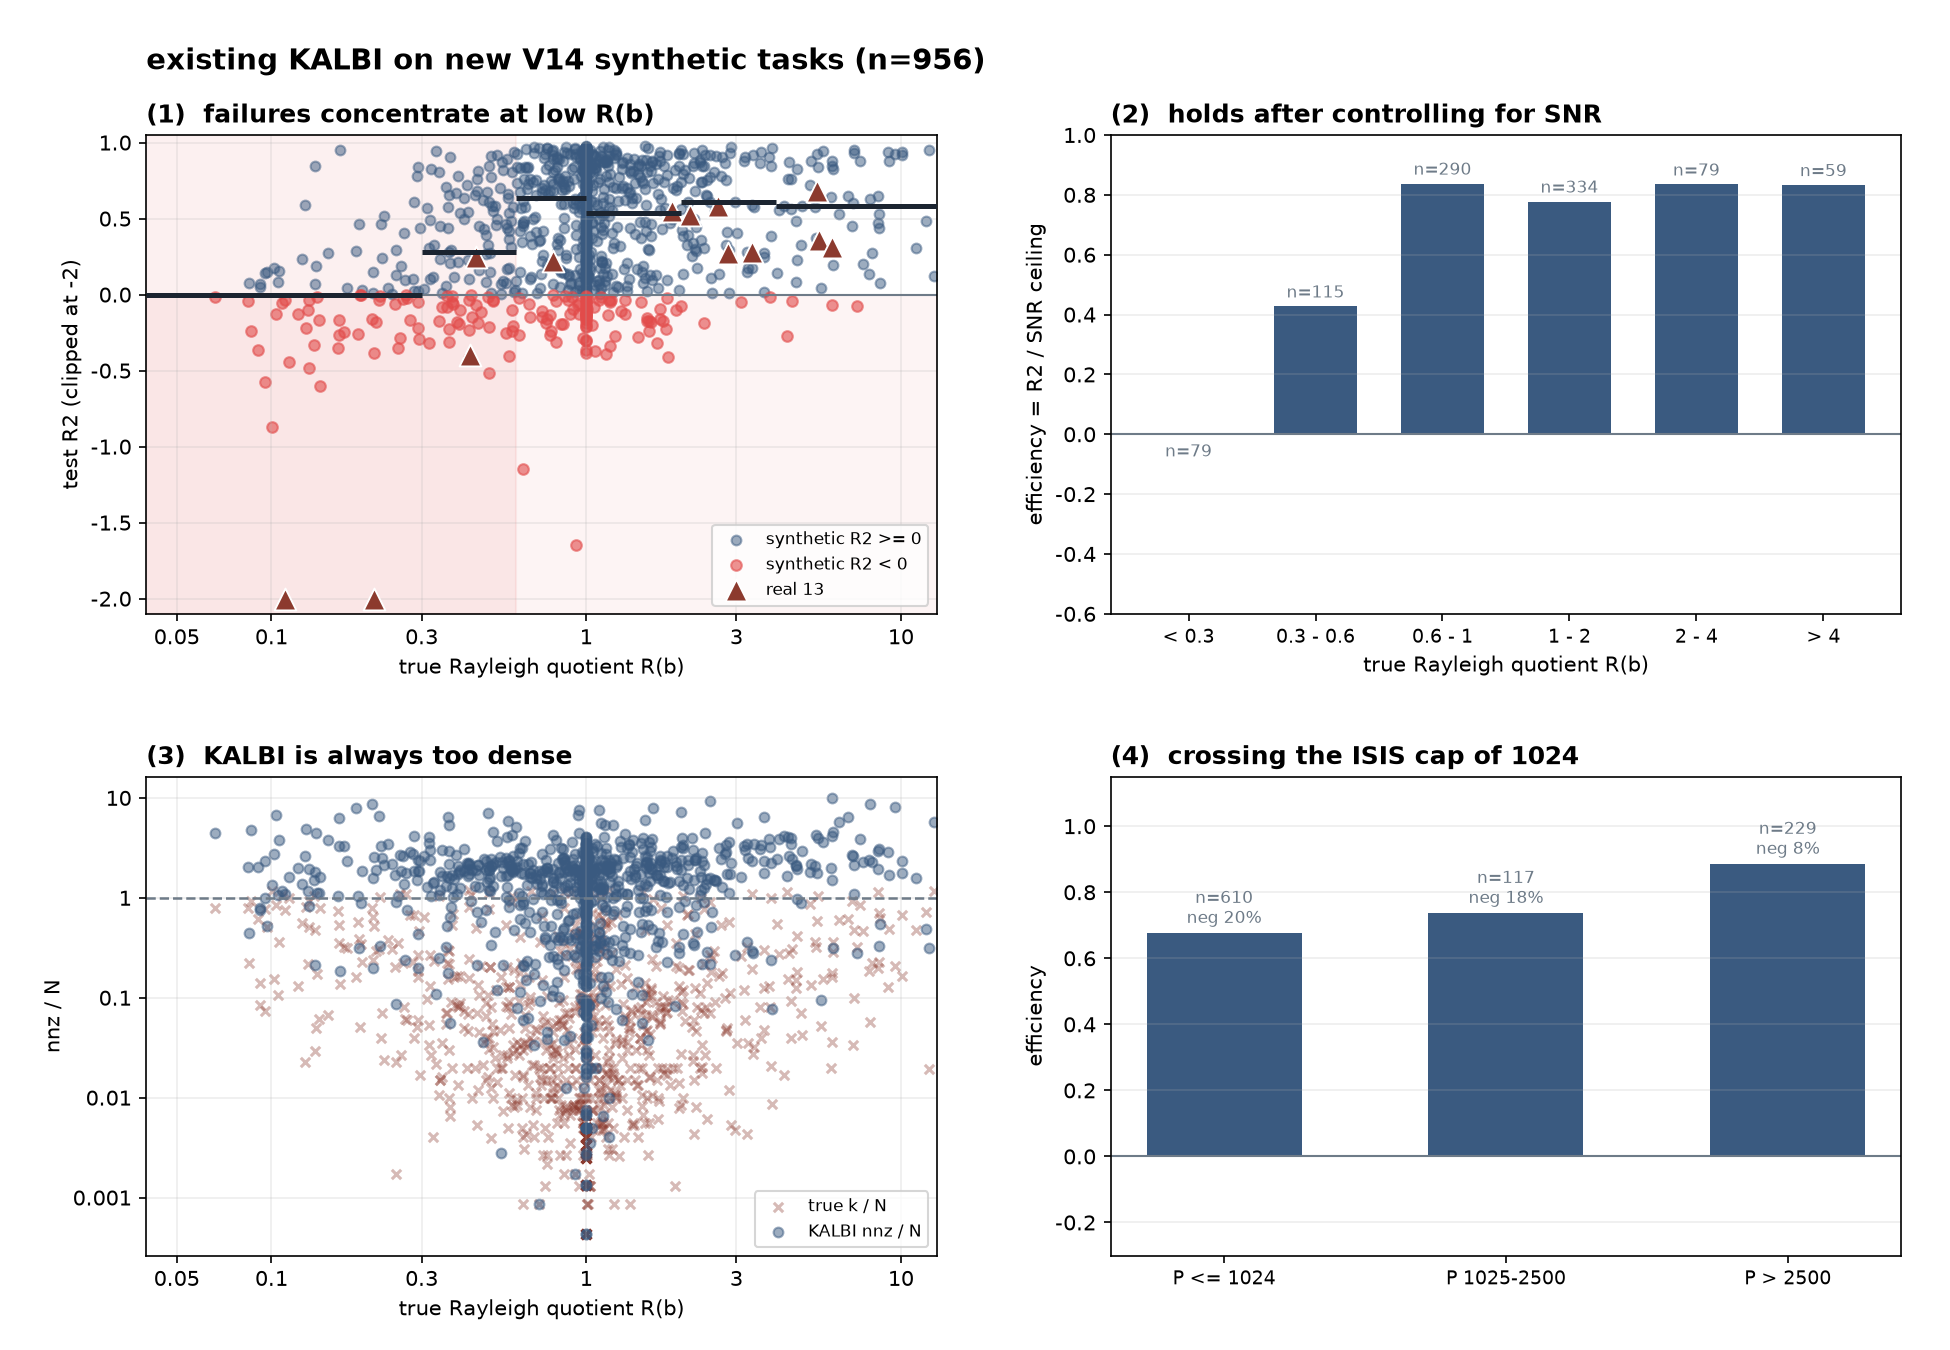
\includegraphics[width=\textwidth]{synth_probe_report_en.png}
\caption{The existing KALBI checkpoint applied to $956$ tasks from the
modified generator; no real data is used except for the overlay.
\textbf{(1)} Test $R^2$ against the Rayleigh quotient. Red points are
negative $R^2$; the shaded band marks $\Rq < 0.6$. Black bars are per-bin
medians. Brown triangles are the thirteen real benchmarks, which fall on the
same curve as the synthetic cloud; the two at $-2$ are clipped from $-2.90$
and $-2.08$. For the synthetic points the abscissa is $\Rtrue$, which we
know; for the real ones it is $R(\bhat)$, which is all that is available.
Since $R(\bhat)$ tracks the truth with slope $0.293$ and has a floor at
$0.425$, the real triangles sit further right than their true position ---
a conservative placement. The vertical stripe at $\Rq = 1$ is the $15\%$ of tasks that
retain the original isotropic sampler, i.e.\ where the old generator lived.
\textbf{(2)} Signal-recovery efficiency $\eta = R^2 / (s/(1+s))$ by bin.
The bar for $\Rq < 0.3$ is invisible because its height is zero.
Efficiency is flat above $0.6$ and collapses only below it --- a threshold,
not a gradient.
\textbf{(3)} Sparsity. Blue is KALBI's $\mathrm{nnz}/N$, red crosses the true
$k/N$; the dashed line is $\mathrm{nnz} = N$. KALBI sits above the line
irrespective of $\Rq$, so over-selection is a fixed habit of the solver
rather than a response to the data.
\textbf{(4)} Efficiency split at the ISIS screening cap of $1024$. Failure
rates fall from $20\%$ to $8\%$, so feature screening is not a separate
failure path.}
\label{fig:panels}
\end{figure}

\paragraph{Difficulty control.}
On the same data and the same splits we also ran CV LASSO ($705$ tasks).

\begin{table}[h]
\centering
\caption{CV LASSO control}
\begin{tabular}{@{}lrrrrr@{}}
\toprule
$\Rtrue$ & $n$ & KALBI $R^2$ & LASSO $R^2$
 & KALBI $R^2<0$ & LASSO $R^2<0$ \\
\midrule
$< 0.3$      &  55 & $0.022$ & $0.069$ & $49\%$ & $25\%$ \\
$0.3$--$0.6$ &  87 & $0.304$ & $0.583$ & $24\%$ & $\phantom{0}8\%$ \\
$0.6$--$1$   & 217 & $0.599$ & $0.705$ & $12\%$ & $\phantom{0}2\%$ \\
$1$--$2$     & 246 & $0.546$ & $0.647$ & $15\%$ & $\phantom{0}1\%$ \\
$2$--$4$     &  56 & $0.669$ & $0.757$ & $\phantom{0}5\%$ & $\phantom{0}0\%$ \\
$> 4$        &  44 & $0.579$ & $0.636$ & $\phantom{0}2\%$ & $\phantom{0}0\%$ \\
\bottomrule
\end{tabular}
\end{table}

For $\Rq \in [0.3, 0.6]$ CV LASSO reaches $R^2 = 0.583$ with an $8\%$ failure
rate. \textbf{In that band the failure is a property of the model, not of the
problem.} Below $0.3$ CV LASSO also degrades ($R^2 = 0.069$, $25\%$
failures), so that region is genuinely hard and we exclude it from the claim.

%==========================================================================
\section{Mechanism: a floor in the output space}

We compared the Rayleigh quotient of the coefficients KALBI \emph{emits}
against the ground truth.

\begin{table}[h]
\centering
\begin{tabular}{@{}rrr@{}}
\toprule
$\Rtrue$ & $R(\bhat)$ & ratio \\
\midrule
$0.188$ & $1.634$ & $8.7$ \\
$0.424$ & $1.640$ & $3.9$ \\
$0.952$ & $1.421$ & $1.5$ \\
$6.057$ & $5.444$ & $0.9$ \\
\bottomrule
\end{tabular}
\end{table}

The log--log regression slope is

\begin{equation}
\frac{d \log R(\bhat)}{d \log \Rtrue} = 0.293
\qquad (\text{perfect tracking would give } 1),
\end{equation}

and the smallest $R(\bhat)$ observed was $0.425$, while the ground truth
reaches $0.090$. \textbf{The required solution does not exist in the model's
output space.} For the group of tasks with median $\Rtrue = 0.359$, KALBI
returns $R(\bhat) = 1.634$.

\paragraph{The same lemma acts twice.}
Where the true quotient is low, KALBI spreads coefficient mass thinly.

\begin{table}[h]
\centering
\begin{tabular}{@{}lrr@{}}
\toprule
 & $\Rtrue < 0.3$ & $0.6$--$1$ \\
\midrule
$\mathrm{nnz}/N$   & $1.95$ & $1.00$ \\
$\max_j|\bhat_j|$  & $0.122$ & $0.540$ \\
\bottomrule
\end{tabular}
\end{table}

Assigning small values to many coordinates \emph{is} an isotropic $\beta$,
and by Proposition~1 an isotropic $\beta$ forces $\Rq \approx 1$.
\textbf{The model reproduces the structural bias of its training data in the
shape of its own output.}

\paragraph{Additional observations.}
Over all $956$ tasks, $\mathrm{nnz} > N$ in $65\%$ of cases ($625$), with a
median over-selection factor of $34\times$ relative to the true support size.
The Direct96 domain $[0,6]$ never reached its cap; the global maximum of
$\max_j|\bhat_j|$ was $1.767$. Splitting by the ISIS screening threshold of
$1024$ gives failure rates of $20\%$, $18\%$ and $8\%$ for
$P \le 1024$, $1025$--$2500$ and $P > 2500$, so feature screening is not a
separate failure path.

%==========================================================================
\section{Numerical identifiability: synthetic and real differ}
\label{sec:stability}

The same checkpoint on the same inputs gave different answers on CPU and on
GPU --- $\mathrm{nnz} = 380$ against $665$, $R^2 = +0.67$ against $-2.08$ ---
while the selected $\lambda$ differed by only $1\%$. Because a $1\%$ input
change should not reorganise the solution, we measured sensitivity directly:
perturb $Z$ by a relative $\varepsilon = 10^{-5}$ and record

\begin{equation}
\text{amplification} \;=\; \frac{\|\Delta\bhat\| / \|\bhat\|}{\varepsilon} .
\end{equation}

A well-posed problem gives $O(1)$; a degenerate one approaches
$1/\varepsilon = 10^5$.

\begin{table}[h]
\centering
\caption{Sensitivity to a $10^{-5}$ relative perturbation of $Z$}
\begin{tabular}{@{}lrrr@{}}
\toprule
 & tasks & median amplification & median $R^2$ spread \\
\midrule
real benchmarks       & 13 & $2.8 \times 10^{4}$ & $0.047$ \\
synthetic, $\Rq < 0.6$ &  9 & $3.3 \times 10^{2}$ & $0.001$ \\
synthetic, $\Rq \ge 0.6$ & 31 & $1.5 \times 10^{2}$ & $0.000$ \\
\bottomrule
\end{tabular}
\end{table}

Two conclusions follow, and they point in opposite directions.

\paragraph{The synthetic evidence is sound.}
Across all six $\Rq$ bins the synthetic amplification stays between $150$ and
$550$ and the $R^2$ spread is $\le 0.001$;
$\mathrm{corr}(\log \Rq, \log \text{amplification}) = -0.09$, i.e.\ no
relationship. The collapse reported in Section~4 is therefore a genuine
failure of the estimator, not an artefact of an ill-posed problem. The
956-task experiment stands.

\paragraph{Real data carries a second, separate pathology.}
On the benchmarks, amplification reaches $5.9 \times 10^{5}$ and the induced
$R^2$ spread is large enough to flip the sign of the headline numbers:
QSAR-TID-10331 moves between $-6.07$ and $+0.69$, QSAR-TID-17080 between
$-2.90$ and $+0.54$, all under a $10^{-5}$ nudge. The minimum eigenvalue of
the selected sub-Gram is numerically negative --- that is, zero to machine
precision --- for five of the thirteen, and
$\mathrm{corr}(\log \lambda_{\min}(G_S), \log \text{amplification}) = -0.74$.
Individual real-data numbers in Table~\ref{tab:real13} should be read as one
draw from a set of near-equivalent solutions, not as point estimates.

\paragraph{Why the generator is immune.}
V14 adds independent featurewise noise before storage,
$v_j \sim \mathrm{Exp}(1)$ and $\epsilon_{ij} \sim N(0, v_j)$, and
restandardises. After that step the Gram acquires a floor,

\begin{equation}
G' = DGD + \operatorname{diag}\!\left(\frac{v_j}{1+v_j}\right)
\qquad\Longrightarrow\qquad
\lambda_{\min}(G') \;\gtrsim\; \min_j \frac{v_j}{1+v_j},
\end{equation}

so the generator can only emit well-conditioned designs. Real data has no
such floor. This is a second generator-to-reality gap, independent of the
Rayleigh quotient, and it has a ready control: the noise rate is currently
fixed at $1$ and is not sampled per task.

%==========================================================================
\section{Generator fix}

The goal is to widen the distribution of $\Rq$. Three changes were made.

\subsection{Relaxed support-size cap}

\begin{verbatim}
max_support = min(p, int(0.60 * (n - 1)))   # was (n - 1) // 3
\end{verbatim}

Driving $\Rq$ below one requires many correlated columns, which the old cap
made impossible. The hard $3k < N$ assertion is replaced by a metadata flag.

\subsection{Eigenvalue targeting}

Draw a target $R^\star$ log-uniformly from $[0.03, 30]$, locate the adjacent
eigenvalue pair with $w_a \le R^\star \le w_b$, and set

\begin{equation}
c_a^2 = \frac{w_b - R^\star}{w_b - w_a},
\qquad
c_b^2 = \frac{R^\star - w_a}{w_b - w_a} .
\end{equation}

Then $c_a^2 + c_b^2 = 1$ and \eqref{eq:weighted} gives $\Rq = R^\star$
exactly. A $15\%$ isotropic component is blended in to avoid a literal
rank-two structure in the eigenbasis. The construction is applied to $85\%$
of tasks and only when $k \le 768$; the remainder keep the original sampler,
so there is no regression risk.

\subsection{Correlated-block supports}

For a random support the sub-Gram saturates at $w_{\max} \approx 2$--$3$, so
large targets are clipped. We instead seed on one column and attach its
$k-1$ highest-correlation partners, producing a cluster that shares a common
factor. Modes are mixed with probability $1/3$ each: random, block, and
half-block.

The $0.95$ correlation filter is not binding. By Gershgorin's theorem,

\begin{equation}
w_{\max} \le 1 + (k-1)\,c ,
\end{equation}

so with $c = 0.95$ and $k = 15$ the bound is $14.3$. In fact $\Rq = 6$ needs
only $15$ columns at equicorrelation $\rho \approx 0.36$: a high Rayleigh
quotient requires a mild common factor, not near-duplicate columns.

\subsection{Result}

\begin{table}[h]
\centering
\caption{Generator before and after the fix (measured on real V14 runs)}
\begin{tabular}{@{}lrr@{}}
\toprule
 & before & after \\
\midrule
$\Rq$ range        & all $\approx 1$ & $0.106$--$8.47$ \\
fraction $\Rq < 1$ & $\approx 0\%$ & $45\%$ \\
fraction $\Rq > 3$ & $0\%$ & $13\%$ \\
$\max \|\beta\|$   & $1.144$ & $3.08$ \\
$\max k$           & $N/3$ & $0.57N$ \\
\bottomrule
\end{tabular}
\end{table}

The real-data range $[0.11, 6.06]$ is now fully contained in the
generator's coverage $[0.106, 8.47]$.

\subsection{Production run}
\label{sec:v15prod}

The corrected generator has since been run to completion: $508$ shards were
produced and admitted to the training pool. Registering them into the rolling
catalogue that the trainer consumes excluded $27$ shards ($5.3\%$), namely
those whose linear-outcome tasks have $3k \ge n$. The exclusion is deliberate.
The trainer's semantic certificate still requires $3k < n$ per task, and we
left that check in force rather than weakening it: it is a genuine statistical
condition on identifiability, not an artefact of the V14 contract. Retaining
it costs little, and the residual figure is itself informative --- only one
task in twenty needed a support larger than $n/3$ to reach its Rayleigh
target. The coverage gain is therefore attributable almost entirely to the
eigenvalue targeting of Section~7.2, with the relaxed cap of Section~7.1
contributing at the margin.

The remaining $481$ shards were distributed over the eight ranks of the
training contract at $60$--$64$ shards each.

\subsection{Problem shape}
\label{sec:v15shape}

V15 inherits V14's shape sampler unchanged; the fix touches only the
coefficient and support side. It is worth recording what that sampler
actually emits, because it does not resemble the evaluation set. Across the
$508$ shards, $n$ has median $1999$ and $p$ has median $10{,}285$, against
$497$ and $988$ for the thirteen benchmarks --- a factor of four in $n$ and
ten in $p$. The cell budget is the binding constraint: $375$ shards ($74\%$)
sit within $0.5\%$ of the \texttt{max\_cells} ceiling of $24$ million, so the
sampler systematically spends its budget, and since $n$ is comparable to real
the budget goes into $p$.

The consequence is that the training and evaluation distributions barely
overlap in shape. Only $45$ shards ($8.9\%$) fall inside the benchmarks'
range of $p$, and only $16$ ($3.1\%$) fall inside both the $n$ and the $p$
range. We record this as an observation rather than a diagnosis: unlike the
$\kappa$ argument of Section~\ref{sec:kappa}, which predicts a measured
quantity on all thirteen benchmarks, nothing here establishes that the shape
mismatch causes the real-data failure. It does, however, bear on
Section~\ref{sec:v15corr}: a design ten times wider dilutes a fixed amount of
correlated structure, so part of V15's lower $q_{99}$ may be attributable to
$p$ rather than to the support-selection mechanism.

\subsection{Correlation structure of the produced data}
\label{sec:v15corr}

The eigenvalue targeting acts on the coefficient vector, not on the design, so
it is worth asking separately whether V15's correlation structure resembles the
benchmarks. We measured pairwise $|\mathrm{corr}|$ on both sources
\emph{after} the $0.95$ filter, which is the state the solver actually sees.

Two caveats govern how the comparison must be read. Computing the full
correlation matrix is infeasible at $p \sim 10^4$, so columns are subsampled to
$300$. Quantiles are unbiased under uniform subsampling and may be compared
directly. The maximum is not: real designs have median $p = 988$ and therefore
sample $9.2\%$ of all pairs, whereas V15 shards run to $p > 4000$ and sample
$0.5\%$, so V15's subsampled maximum understates its true one by much more.
For the maximum we therefore use the exact per-shard value the generator
records.

\begin{table}[h]
\centering
\caption{Pairwise $|\mathrm{corr}|$ after the $0.95$ filter. Medians across
datasets or shards. The first two rows are directly comparable; the third
uses the generator's exact audit on all $508$ shards against the real
subsampled maximum.}
\label{tab:corr}
\begin{tabular}{@{}lrrr@{}}
\toprule
 & real ($13$) & V15 & ratio \\
\midrule
median $|\mathrm{corr}|$   & $0.0278$ & $0.0230$ & $1.2$ \\
$95$th pct                 & $0.1736$ & $0.0888$ & $2.0$ \\
max (exact)                & $0.9248$ & $0.8498$ & $1.1$ \\
\bottomrule
\end{tabular}
\end{table}

Three things follow. First, the filter is honoured exactly: none of the $508$
shards exceeds $0.95$ on either the exact or the sampled audit. Second, the
bulk of the distribution already matches --- the typical pair is as weakly
correlated in V15 as in the benchmarks. Third, the gap is confined to the
upper-middle of the distribution, where V15's $95$th percentile is half of
real; yet the extremes do reach the filter edge, with the exact maximum having
$95$th percentile $0.9128$ and maximum $0.9381$.

This shape follows from the construction. The \texttt{correlated\_block}
support mode attaches a seed column's highest-correlation partners, which
manufactures a handful of near-collinear pairs, while the remainder of the SCM
design stays close to independent. Real designs instead carry a thick band of
moderately correlated columns. The consequence is that V15 closes the $\Rq$
coverage gap without reproducing that band, which is consistent with the
amplification gap of Section~\ref{sec:stability} being a separate axis from
the $\Rq$ gap, and gives that observation its first quantitative handle.

\begin{figure}[h]
\centering
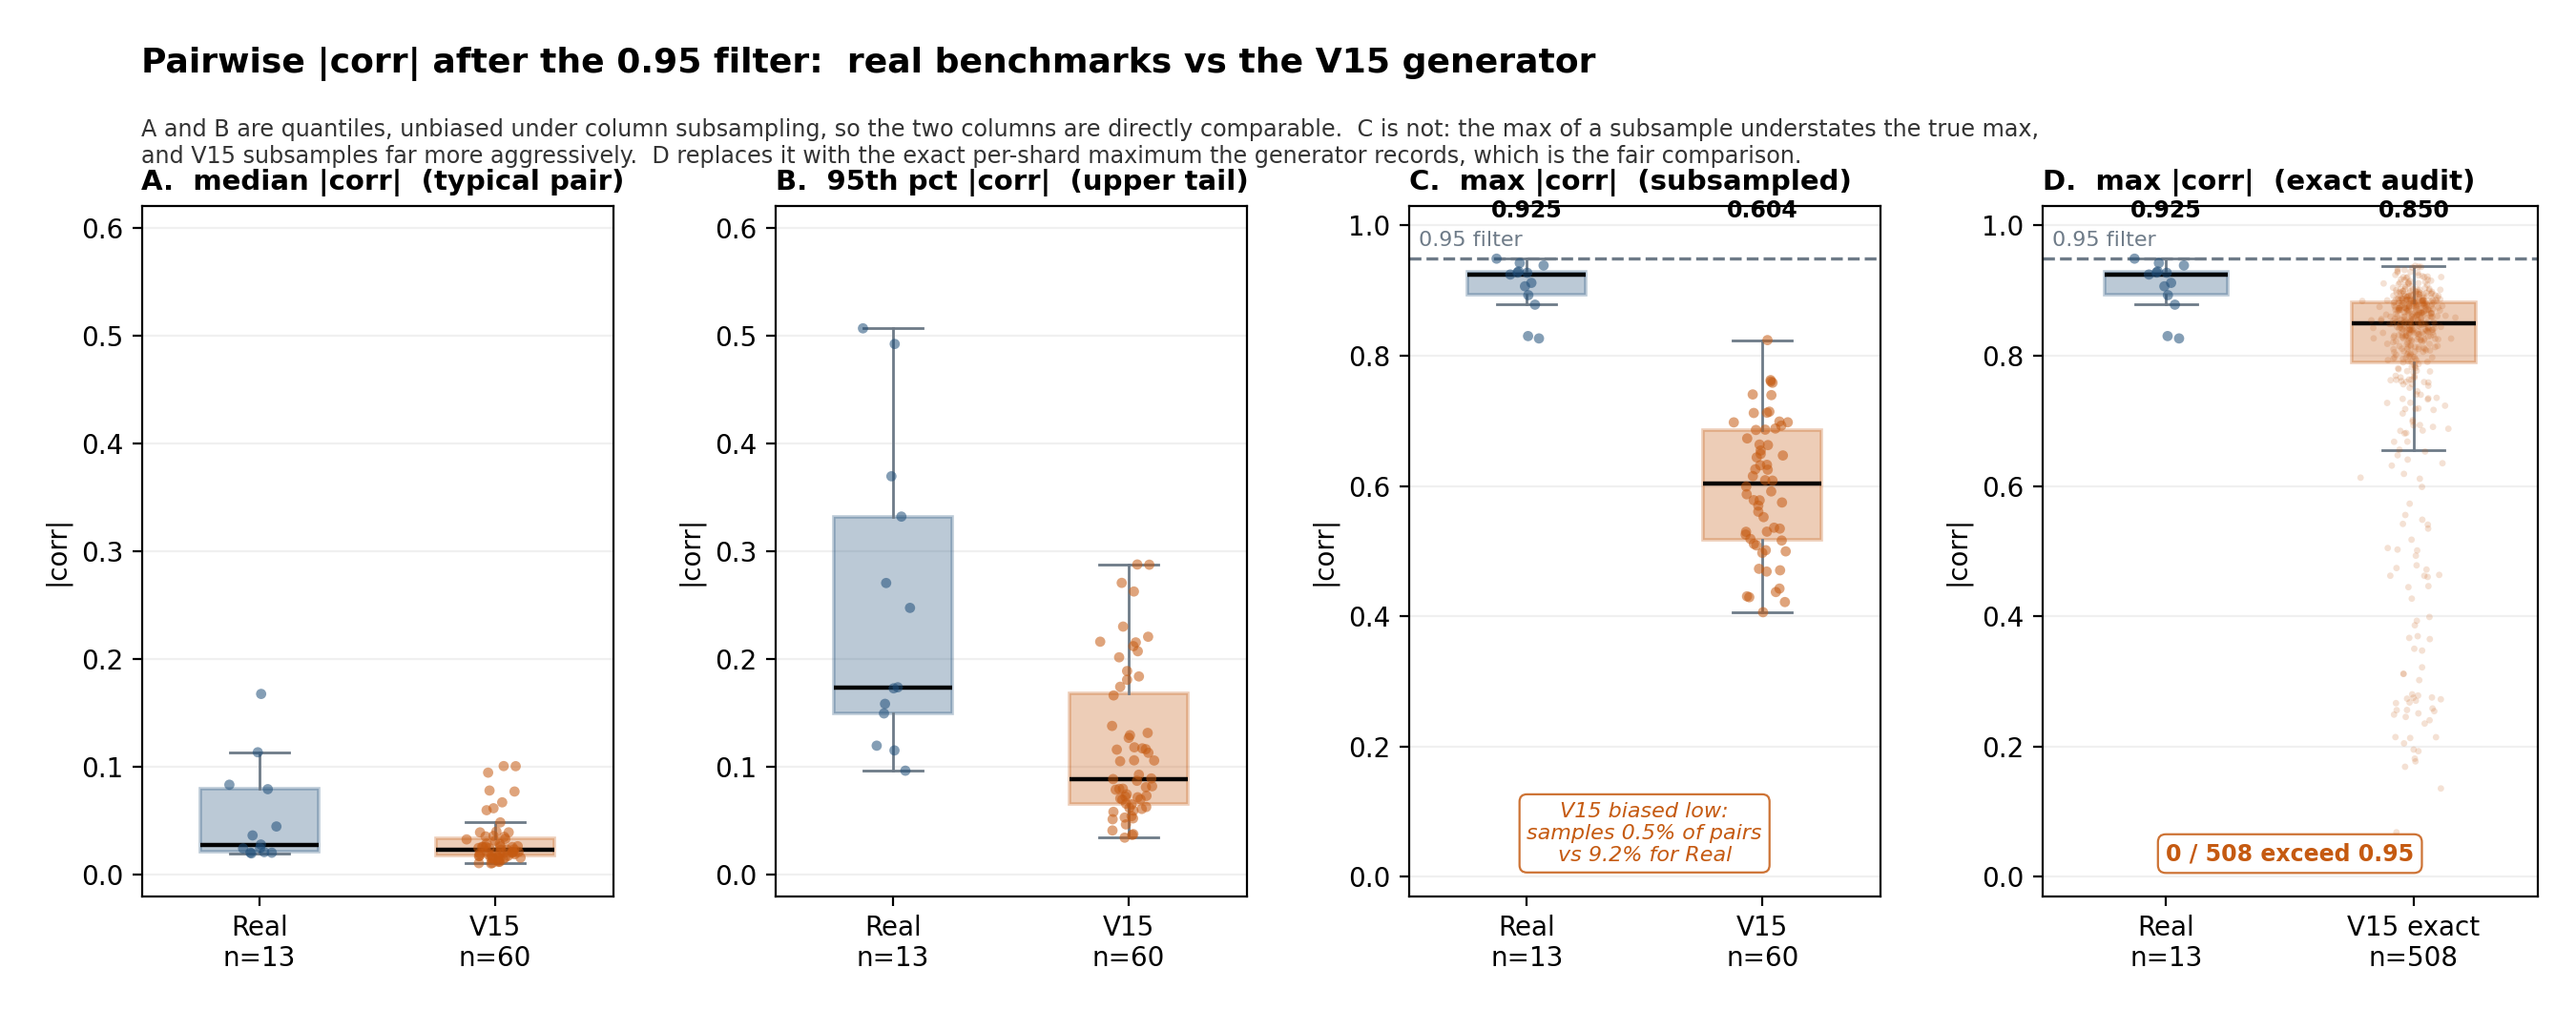
\includegraphics[width=\textwidth]{corr_box.png}
\caption{Pairwise $|\mathrm{corr}|$ after the $0.95$ filter, one point per
dataset or shard. Panels A and B are quantiles and so are unbiased under the
column subsampling both sources undergo. Panel C is the maximum under the same
subsampling and is \emph{not} comparable, because V15 samples $0.5\%$ of pairs
against real's $9.2\%$; panel D replaces it with the exact per-shard maximum
the generator records on all $508$ shards.}
\label{fig:corrbox}
\end{figure}

Plotting the correlation matrices directly shows what the percentile gap looks
like (Figure~\ref{fig:corrheat}). Across the same columns and a shared colour
scale, the real panels carry visible block and band texture while typical V15
panels are nearly blank away from the diagonal.

To see whether this is representative we extracted all $508$ shards and all
thirteen benchmarks (Figure~\ref{fig:corrheatall}), summarising each panel by
$q_{99}$, the $99$th percentile of its off-diagonal $|\mathrm{corr}|$. The
full sweep corrects the impression a small sample gives. Real spans
$0.219$--$0.913$ with median $0.416$; V15 spans $0.052$--$0.584$ with median
$0.154$. V15's maximum therefore exceeds eleven of the thirteen benchmarks ---
only \texttt{mtp2} ($0.913$) and \texttt{Acute\_Myeloid\_Leukemia} ($0.710$)
lie above it --- and $137$ shards ($27\%$) exceed the least correlated
benchmark. But only $14$ shards ($2.8\%$) reach real's median.

The deficit is thus one of frequency rather than of reach. The generator can
already produce designs as correlated as most of the benchmarks; it simply
produces them rarely, because \texttt{correlated\_block} is drawn with
probability $1/3$ and acts only on the support. Closing the gap therefore
looks like a change of sampling weights, not a new mechanism --- which is a
much cheaper intervention than the one Section~\ref{sec:stability} anticipated.

\begin{figure}[h]
\centering
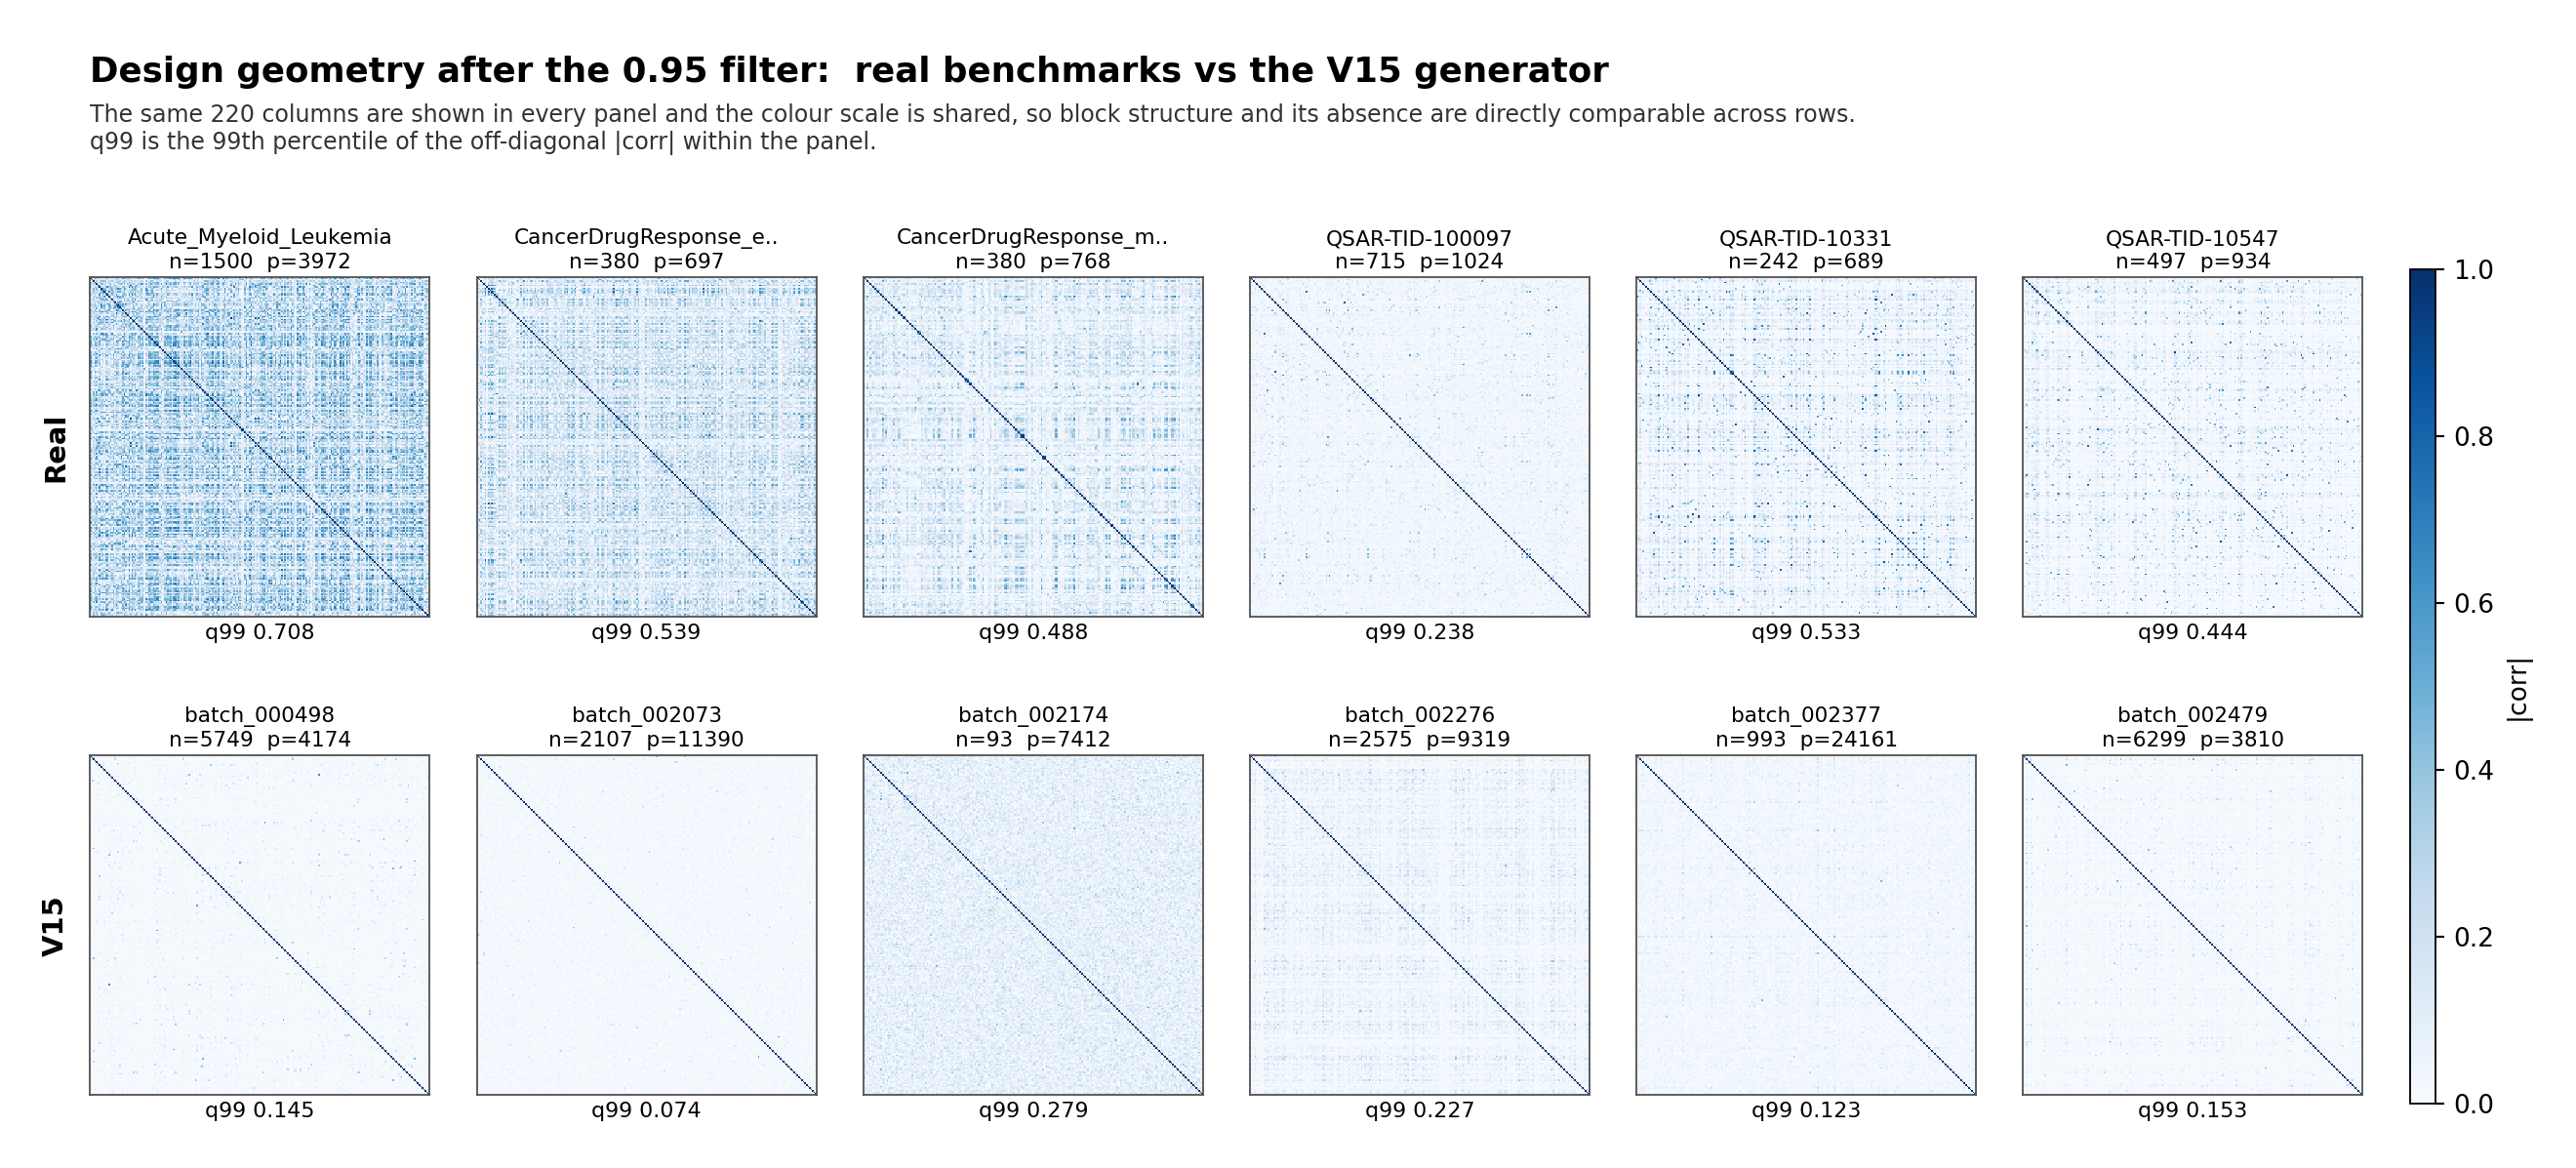
\includegraphics[width=\textwidth]{corr_heatmap.png}
\caption{Design geometry after the $0.95$ filter, six benchmarks against six
shards. The same $220$ columns and the same colour scale in every panel;
$q_{99}$ is the $99$th percentile of the off-diagonal $|\mathrm{corr}|$
within each panel.}
\label{fig:corrheat}
\end{figure}

\begin{figure}[h]
\centering
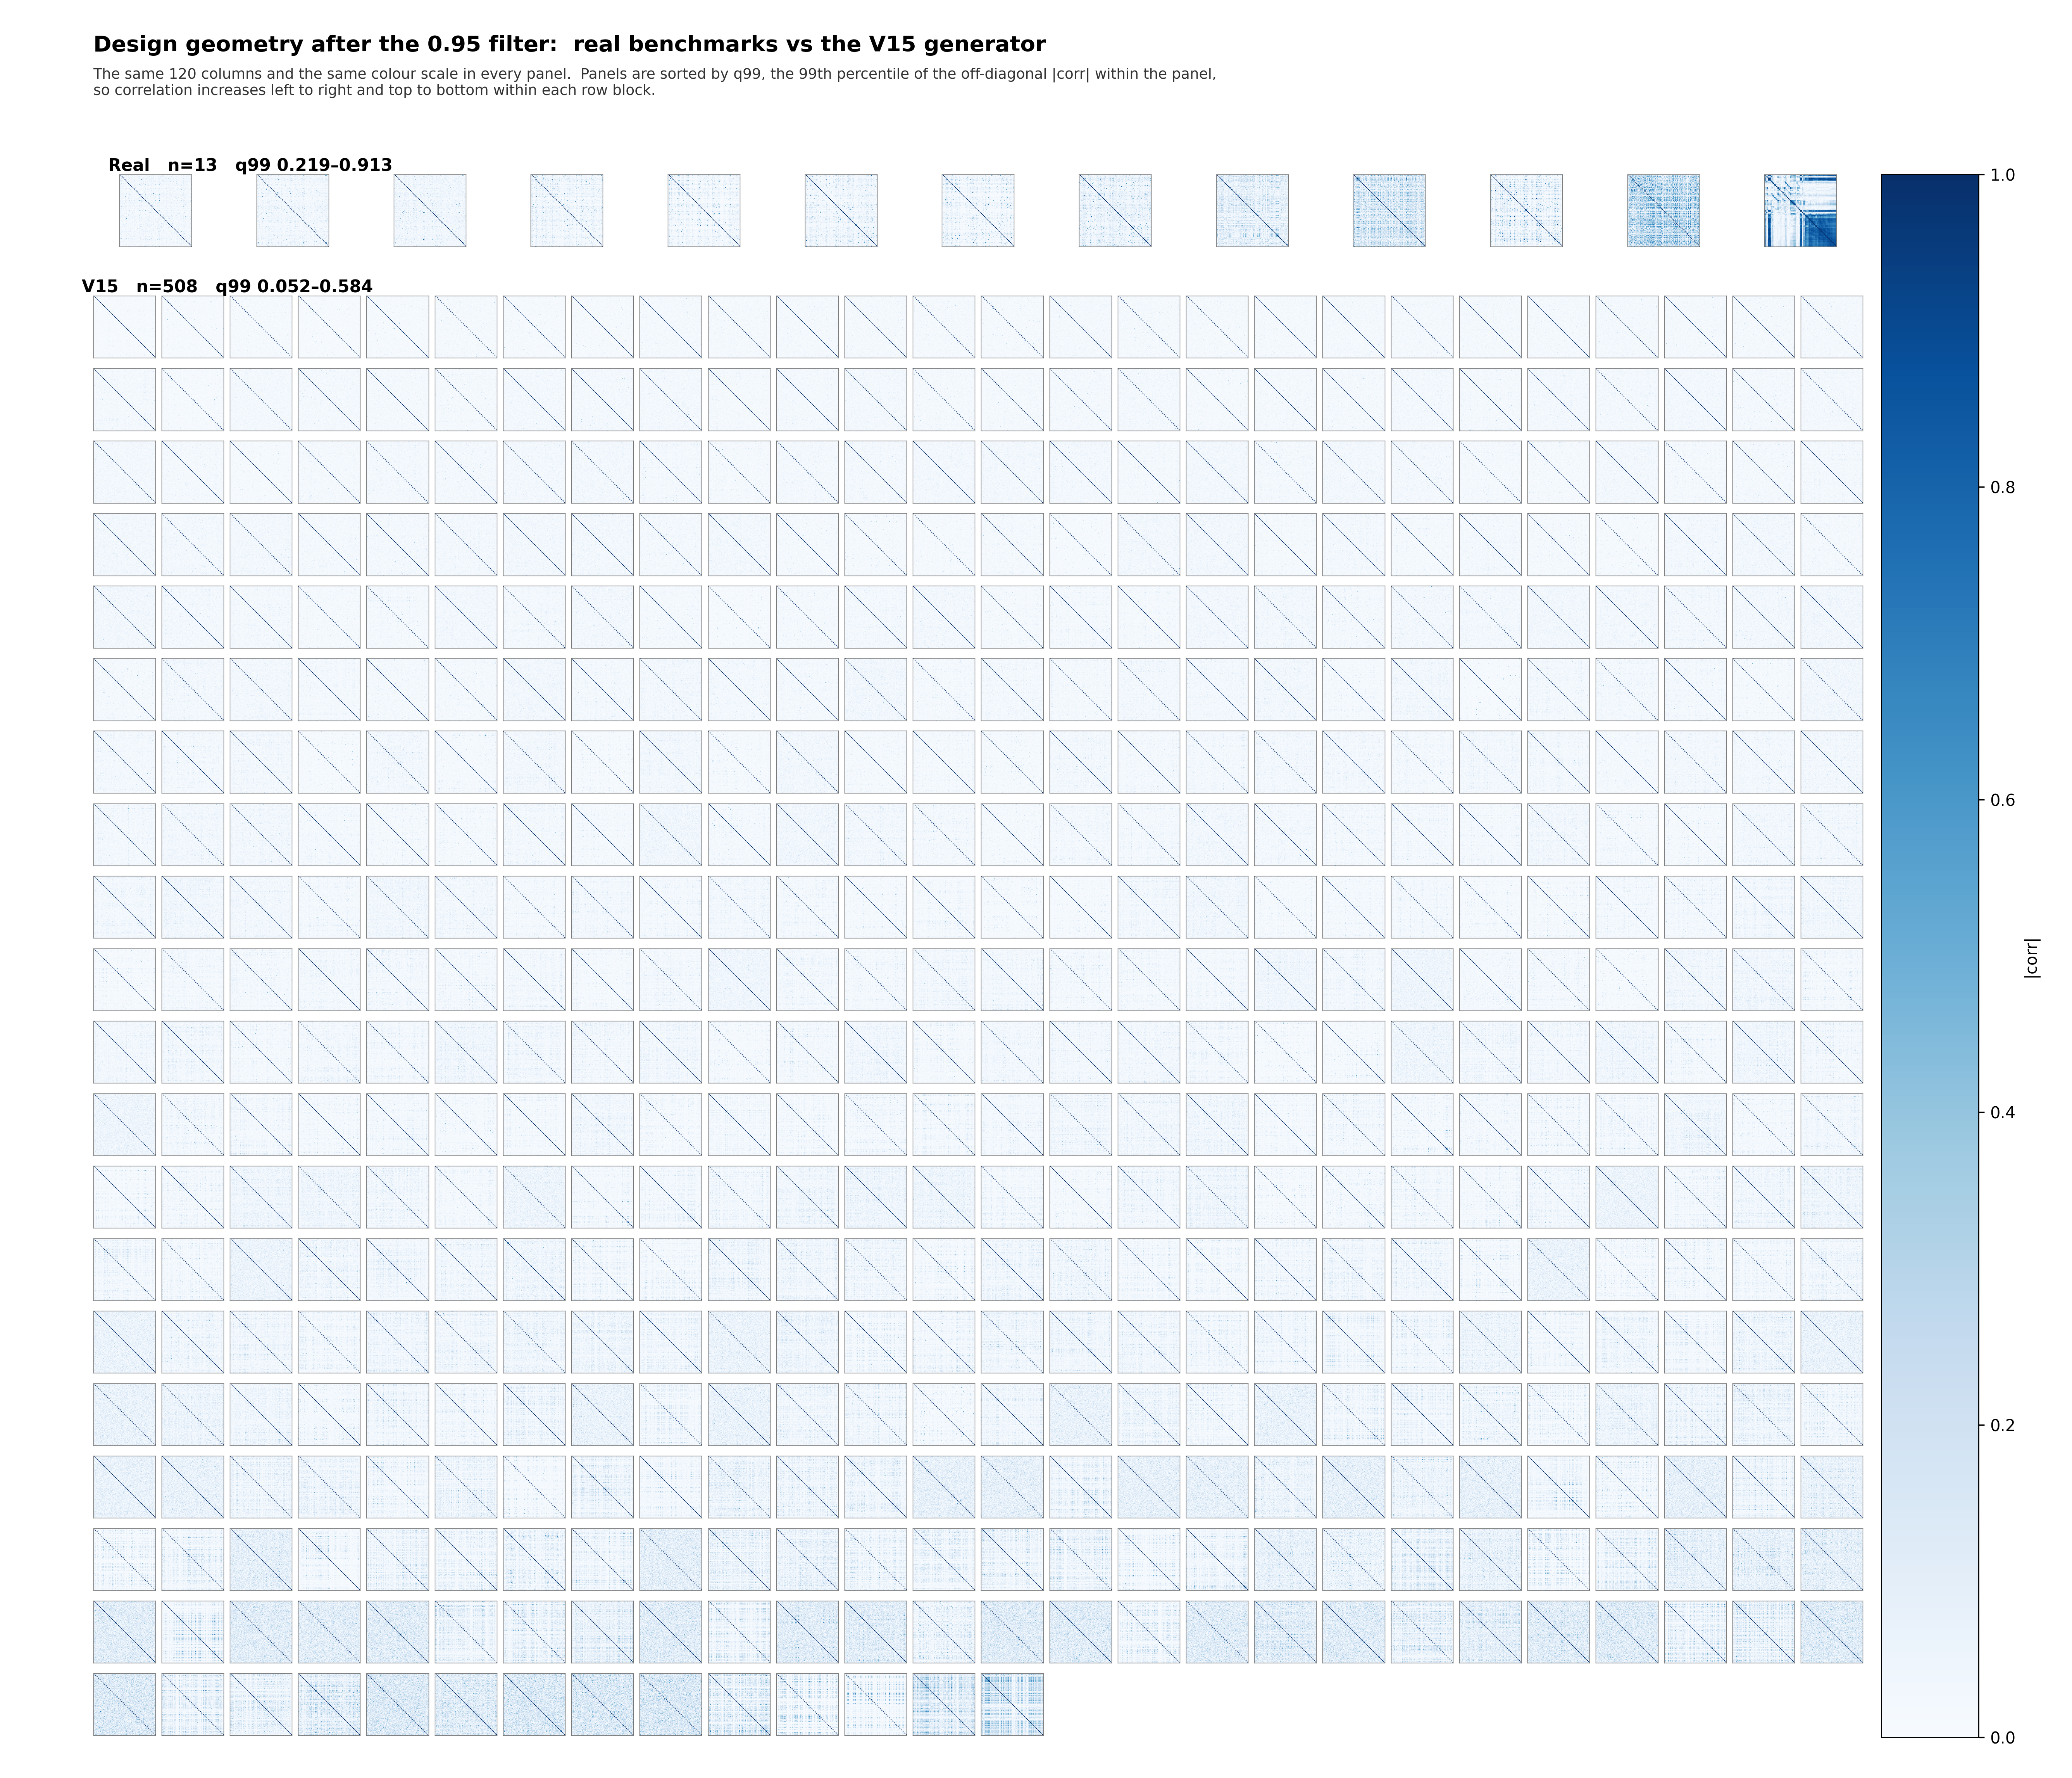
\includegraphics[width=\textwidth]{corr_heatmap_all.png}
\caption{All thirteen benchmarks and all $508$ shards, $120$ columns per
panel, sorted by $q_{99}$ so that correlation increases towards the lower
right of each block. The V15 block reaches real's range at its upper end but
concentrates far below it.}
\label{fig:corrheatall}
\end{figure}

\subsection{Retraining pipeline}
\label{sec:pipeline}

Migrating the frozen-beta selector run from V14 to V15 data is not a change of
one path. The trainer verifies the data pipeline at several independent
layers, and each had to be brought forward honestly rather than disabled:

\begin{enumerate}
\itemsep2pt
\item \textbf{Contract strings and generator hash.} Three constants
      (\texttt{SCM\_CONTRACTS["tabicl\_v2"]},
      \texttt{LINEAR\_TASK\_TARGET\_CONTRACT}, \texttt{V14\_GENERATOR\_SHA256})
      were repointed to the values the V15 generator actually emits. The SNR
      contract, its bounds and the five regime names were already
      character-identical and were left untouched.
\item \textbf{Per-task semantic certificates.} Each catalogue entry carries the
      eight linear-outcome fields the batcher indexes unconditionally
      (support size and fraction, support and coefficient and error family
      identifiers, SNR regime, target and realised SNR). These are read
      directly from the shards rather than from a manifest, so the certificate
      records measured values.
\item \textbf{Resume contract.} Two entries were removed from the resume
      equality check, \texttt{source\_hashes} and
      \texttt{exact\_training\_arguments}, both of which change by
      construction when the data pipeline is deliberately replaced. World
      size, trainer version, checkpoint version and every contract version
      remain strictly checked.
\item \textbf{Checkpoint continuity.} The checkpoint's frozen catalogue
      snapshot was replaced with the V15 catalogue and the per-rank stream
      state was cleared, so the run resumes the \emph{weights} of the
      reinitialised checkpoint while drawing a fresh task stream. The
      canonical penalty cache is bound by absolute path and was restored at
      the path the checkpoint records.
\end{enumerate}

With these in place a $100$-step smoke run completed on eight ranks, from
selector step $30{,}000$ to $30{,}100$, in $434$ seconds ($4.34$\,s per step).
It terminated cleanly, wrote a checkpoint and passed the reload verification.

\subsection{The constraint holds under training}
\label{sec:kappa_under_training}

The smoke run supplies the first evidence that the construction of
Section~\ref{sec:monotone} survives gradient updates rather than merely
holding at initialisation. The trainer logs $\rho'(0)$ and $\max\rho'$
separately per rank; after $100$ updates they agree to the printed precision
on every rank, for example

\begin{center}
\begin{tabular}{@{}lrr@{}}
\toprule
 & rank $6$ & rank $7$ \\
\midrule
$\max_{\text{task}} \rho'(0)$   & $11.443906784057617$ & $12.797087669372559$ \\
$\max_{\text{task}} \max\rho'$  & $11.443906784057617$ & $12.797087669372559$ \\
$\min_{\text{task}} \rho'(0)$   & $4.043909549713135$  & $4.493143558502197$ \\
$\min_{\text{task}} \max\rho'$  & $4.043909549713135$  & $4.493143558502197$ \\
\bottomrule
\end{tabular}
\end{center}

so $\kappa = 1$ exactly. The normalisation is likewise intact: the maximum
error in $\rho(6) = 1$ is $6.0 \times 10^{-8}$ and in $\rho(0) = 0$ is zero,
and $\min \rho' = 1.6 \times 10^{-7} > 0$. The frozen-beta regime is confirmed
by $0$ trainable beta parameters and $0$ parameters carrying gradients, and
the selector updated on all $100$ steps with no zero-gradient skips.

One quantity deserves attention in the longer run. The per-task $d_0$ now
spans $4.04$--$12.80$, above the useful range $[0.167, 8]$ established from the
cache decode in Section~\ref{sec:monotone} and well above the reinitialisation
value of $2.653$. An increase is the expected direction, since the threshold
requires $d_0 e^{\ell} \gtrsim 1$ and the free selector was starving it. But it
is also the direction of the degenerate hard-threshold solution that motivated
reinitialising the penalty head in the first place. One hundred steps cannot
distinguish the two, and $d_0$ should therefore be read alongside
Table~\ref{tab:criteria} in the $2000$-step run.

Extrapolating from the measured step time, the $2000$-step run requires
$2.4$ hours and the full $30{,}000$-step run $36$ hours.

%==========================================================================
\section{An invariant the architecture states but never enforces}
\label{sec:kappa}

Sections~\ref{sec:stability} and~7 establish that V14 emits only
well-conditioned designs and that the fix restores coverage. They do not
explain \emph{how} that training distribution damages the selector. This
section supplies the mechanism, and it is not a tuning problem but a broken
invariant.

\subsection{The Direct96 contract}

The selector emits $96$ parameters that are decoded into a penalty derivative
on a fixed non-uniform grid on $[0,6]$,
%
\begin{equation}
\rho'(t) \;=\; c \;+\; \sum_{k=1}^{95} w_k \max(t - t_k,\, 0),
\label{eq:hinge}
\end{equation}
%
followed by a positivity map and normalisation of the \emph{area},
$\int_0^6 \rho'(t)\,dt = 1$, i.e.\ $\rho(6) = 1$. Note what is \emph{not}
constrained: the hinge weights $w_k$ are free in sign, and the hinge functions
$\max(t-t_k,0)$ are non-decreasing. A positive $w_k$ therefore makes $\rho'$
\emph{increase} after $t_k$, and because only the area is pinned, a derivative
that rises and then falls satisfies the contract exactly.

Two quantities govern the solution. The zero-KKT threshold is set by
$\rho'(0) \equiv d_0$: coordinate $j$ is held at zero when
$|X_j^\top r|/N \le \lambda d_0$. The $\lambda$ scale, however, is set
elsewhere. In \texttt{selector\_v20\_yconditioned.py:144},

\begin{verbatim}
def _lambda_reference_slope(self, encoded):
    """Use the maximum penalty force over the bounded Direct96 domain.

    Direct96 fixes rho(6)=1, so max rho' is strictly positive and has a
    stable scale.  It equals d0 for the usual L1/SCAD/MCP-like decreasing
    derivative paths, while remaining valid for ridge-like paths with
    d0 approximately zero.
    """
    return encoded["drho"].amax(dim=-1)
\end{verbatim}

The docstring states the assumption outright: $\max\rho'$ ``equals \texttt{d0}
for the usual L1/SCAD/MCP-like \emph{decreasing} derivative paths.'' That is
exactly
%
\begin{equation}
\kappa \;\equiv\; \frac{\rho'(0)}{\max_t \rho'(t)} \;=\; 1 ,
\label{eq:kappa}
\end{equation}
%
which holds for every classical penalty, since LASSO has $\rho'$ constant and
SCAD and MCP have $\rho'$ maximal at the origin. Nothing in the
parameterisation of~\eqref{eq:hinge} enforces it.

The same file computes the violation and discards it, at line $599$ of
\texttt{selector\_v24\_}\allowbreak\texttt{additive512\_}\allowbreak%
\texttt{trajectory.py}:

\begin{verbatim}
concavity = (
    encoded["drho"][..., 1:] - encoded["drho"][..., :-1] > 1e-7
).float().mean(-1)
...
"penalty_concavity_violation_fraction": concavity,
\end{verbatim}

\noindent the fraction of grid intervals on which $\rho'$ increases is
recorded for logging and never enters the loss. Eight lines later the
consequence is visible in the code itself:

\begin{verbatim}
"zero_kkt_ratio": raw_lambda * d0       / lambda_max_safe,
"force_ratio":    raw_lambda * max_drho / lambda_max_safe,
\end{verbatim}

\noindent two ratios that coincide precisely when $\kappa = 1$ are carried as
separate quantities.

\subsection{Measurement}

Table~\ref{tab:kappa} reports the penalty the trained selector actually
chooses on the thirteen benchmarks.

\begin{table}[h]
\centering
\caption{Learned penalty shape on the thirteen real benchmarks.
$\ell$ is the learned log threshold multiplier, so the effective threshold is
$\tau_j = \lambda\, d_0 e^{\ell_j} / g_j$.}
\label{tab:kappa}
\begin{tabular}{@{}lrrr@{}}
\toprule
 & median & min & classical value \\
\midrule
$\kappa = \rho'(0)/\max\rho'$ & $0.109$ & $0.030$ & $1$ \\
$\rho'(6)$                    & $0.0000$ & --- & $>0$ (LASSO) \\
$d_0$                         & $0.417$ & --- & $1/6$ (LASSO) \\
$e^{\ell}$                    & $0.831$ & --- & --- \\
$d_0 e^{\ell}$                & $0.338$ & --- & --- \\
\bottomrule
\end{tabular}
\end{table}

These figures are reproducible. Across two independent re-measurements every
per-dataset value is bit-identical, so the decode path itself is deterministic.
One anomaly is worth recording: on one of the two runs TID-10980 aborted with
\texttt{Direct96 proposal contains nonfinite values} and succeeded on the
other. Dropping it moves the medians to $\kappa = 0.102$ and $d_0 = 0.393$,
which is how much a single dataset matters at $N = 13$. The failure is
intermittent rather than systematic and is of the same character as the
reproducibility issue documented in Section~\ref{sec:stability}.

The learned derivative is a bump: approximately zero at the origin, peaking at
$t \in [0.15, 0.45]$, and identically zero beyond $t \approx 0.5$ on all
thirteen. Three consequences follow directly.

\begin{enumerate}
\itemsep2pt
\item \textbf{No thresholding force.} With $\kappa \approx 0.1$ the $\lambda$
      scale is calibrated against a slope nine times larger than the one that
      actually thresholds, so raising $\lambda$ does not drive coefficients to
      zero. Empirically $\mathrm{nnz} > N$ on seven of thirteen.
\item \textbf{The force is applied where it cannot create sparsity.}
      Section~\ref{sec:real} records $\max_j |\bhat_j| \le 0.447$ across all
      thirteen, so every coefficient lies inside $[0, 0.45]$ --- precisely the
      interval on which the bump attains its maximum. The learned penalty
      therefore shrinks the mid-range hard while exerting almost no force at
      the origin, which is the opposite of what produces a sparse solution.
      That $\rho'(6) = 0$ on all thirteen would additionally leave large
      coefficients unpenalised, but no coefficient reaches that regime here,
      so the operative defect is the missing threshold alone.
\item \textbf{An exact prediction.} At $\lambda = \lambda_{\max}$ the solution
      should be identically zero, which requires $d_0 e^{\ell} \gtrsim 1$.
      This inequality holds on exactly two datasets (TID-100097 at $3.587$ and
      TID-10929 at $1.425$) and fails on the other eleven, and it predicts
      $\mathrm{nnz}(\lambda_{\max}) = 0$ correctly on \textbf{all thirteen}.
\end{enumerate}

\subsection{Why training selects this shape}

The selector's objective is held-out mean squared error alone. On the designs
V14 emits, $\Rq \approx 1$ and the Gram matrix is well conditioned
(Section~\ref{sec:stability}), so a dense, ridge-like solution is never
punished on held-out rows. A penalty that fails to threshold therefore costs
nothing during training. Real data spans $\Rq \in [0.11, 6.06]$, where the
same solution is catastrophic. The generator defect of Sections~2--7 and the
invariant violation of this section are the same failure seen from two ends:
V14 removed the pressure that would have forced $\kappa \to 1$.

%==========================================================================
\section{Existence: classical penalties solve all thirteen}
\label{sec:family}

The preceding argument implicates the selector. It does not by itself show
that the rest of the system is sound, and that distinction decides whether
retraining is worth the compute.

The Direct96 encoder \texttt{native196\_from\_derivative\_knots} accepts an
\emph{arbitrary} derivative sampled on the grid and returns the feature vector
and $d_0$ that the solver consumes. We therefore construct LASSO, MCP$(\gamma)$
and SCAD$(a)$ analytically, area-normalise them to $\rho(6)=1$, and pass them
directly to the \textbf{frozen} beta solver, bypassing the selector entirely.
Because $d_0$ differs across shapes, $\lambda$ is swept as
$\lambda = r\,\lambda_{\max}/d_0$ so that $r$ is a comparable zero-KKT ratio;
$r = 1$ should annihilate the solution for every shape. Nine shapes times
forty values of $r$ gives $360$ solves per dataset from a single encoding pass.

\begin{table}[h]
\centering
\caption{Frozen solver with classical penalties. ``best'' is the maximum over
the $9 \times 40$ grid and ``LASSO'' restricts to $\rho' \equiv \mathrm{const}$;
both select $r$ on the test split and are therefore oracles.}
\label{tab:family}
\begin{tabular}{@{}lrrr@{}}
\toprule
 & selector & LASSO only & best of nine \\
\midrule
QSAR-TID-10331 & $-2.084$ & $+0.354$ & $+0.376$ \\
QSAR-TID-17080 & $-2.899$ & $+0.125$ & $+0.167$ \\
QSAR-TID-10547 & $-0.394$ & $+0.226$ & $+0.258$ \\
\midrule
median $R^2$   & $+0.281$ & $+0.367$ & $+0.376$ \\
$R^2 < 0$      & $3/13$   & $0/13$   & $0/13$ \\
\bottomrule
\end{tabular}
\end{table}

Every dataset is recovered, including the three on which the selector produces
$R^2$ below $-0.39$. Since the solver weights, the encoder, the correlation
filter and the standardisation are identical across the two columns, none of
them can be responsible. The defect is the selector's penalty shape together
with its $\lambda$.

Two qualifications matter and we state them before drawing the conclusion.
First, $r$ is chosen on the test split, so Table~\ref{tab:family} is an upper
bound: it establishes that a solution \emph{exists} inside the monotone family,
not that it can be found from training data alone. Second, plain LASSO attains
$+0.367$ against $+0.376$ for the best of nine, so the entire learned
$96$-dimensional penalty apparatus is currently worth $0.009$ in median
$R^2$ --- and, as measured, considerably less than nothing.

The shapes that win are spread across the family (MCP$(0.5)$ on three
datasets, MCP$(4)$, SCAD$(3.7)$, SCAD$(6)$ and LASSO on two each, MCP$(0.25)$
and MCP$(2)$ on one), and under $\rho(6)=1$ their $d_0$ values run from
$0.167$ (LASSO) to $8.0$ (MCP$(0.25)$). The useful range of $d_0$ is thus
$[0.167, 8]$, a fact we use in Section~\ref{sec:monotone}.

A residual anomaly is worth recording. At $r = 1$ the solution should be
empty, and it is on nine of thirteen, but four retain support:
TID-10331 ($180$), TID-17080 ($299$), TID-10547 ($92$) and mtp2 ($41$). These
are precisely the datasets with the largest perturbation amplification in
Section~\ref{sec:stability}. Since the penalty is exactly LASSO in that
column, this cannot be a shape defect; the likely cause is the fixed budget of
ten proximal steps failing to converge on ill-conditioned designs. Retraining
the selector will not address it.

%==========================================================================
\section{A structural fix and its verification}
\label{sec:monotone}

\subsection{Construction}

The hinge functions in~\eqref{eq:hinge} are non-decreasing, so forcing the
weights negative makes $\rho'$ non-increasing:
%
\begin{equation}
w_k \;=\; -\,\mathrm{squareplus}(\theta_k) \;<\; 0
\quad\Longrightarrow\quad
\rho'(t_1) \ge \rho'(t_2) \ \ \text{for } t_1 \le t_2 .
\label{eq:monotone}
\end{equation}
%
The positivity map is monotone increasing and therefore preserves the
ordering, and the area normalisation is left untouched, so $\rho(6) = 1$ and
the $\lambda$ scale contract are unchanged. Three properties follow by
construction rather than by penalty term:
$\rho'$ non-increasing (hence $\rho$ concave, the standard regularity
condition); $\rho'(0) = \max\rho'$, i.e.\ $\kappa = 1$ and the two ratios of
Section~\ref{sec:kappa} coincide; and $\rho'(0) \ge 1/6$. LASSO, SCAD and MCP
all lie inside the restricted family, as Table~\ref{tab:family} confirms
operationally. The squareplus map is used rather than a ReLU because its
Jacobian is nonzero on the whole line, so gradients survive for weights driven
far negative.

\subsection{Where the constraint may be applied}

The patch cannot go into \texttt{canonical\_penalty.py}. The $300$k penalty
cache validates a sha256 closure over its source files, and that file is a
member:

\begin{verbatim}
expected_sources = {
    "generator":              generate_canonical_penalty_cache.py,
    "canonical_builder":      canonical_penalty.py,
    "penalty_sampler_v9":     penalty_sampler_v9.py,
    "penalty_relu_converter": penalty_relu_mlp_pwl_v33.py,
}
\end{verbatim}

Editing it by a single byte aborts cache loading with
\texttt{canonical cache source hash mismatch}, which we observed.
\texttt{selector\_v11\_canonical.py} is not in the closure, and the training
script records its hash for provenance only.

Applying the constraint in the selector head is also the correct choice on its
merits. Cache penalties reach the solver through
\texttt{CanonicalPenaltyCache.encoded\_indices}, which calls the unmodified
builder directly; that free-form distribution is what the \emph{frozen} beta
solver was trained on, and narrowing it would push a frozen network
out of distribution. The diagnosed defect concerns only the selector's
proposal, so only the selector's decode path is constrained.

\subsection{Verification}

Table~\ref{tab:verify} reports the checks that must pass before any training
run. The distribution of $d_0$ is the substantive one: what matters is not the
behaviour under isotropic Gaussian latents but under the calibrated map
$\text{proposal} = \mu_{\mathrm{cache}} + \sigma_{\mathrm{cache}} \odot
\text{raw}$ that the network actually traverses. We therefore decode $20{,}000$
parameter vectors drawn from the cache itself.

\begin{table}[h]
\centering
\caption{Verification of the monotone constraint. Structural checks are exact;
the $d_0$ distribution is measured on $20{,}000$ cache parameter vectors.}
\label{tab:verify}
\begin{tabular}{@{}lr@{}}
\toprule
check & result \\
\midrule
$\rho'$ non-increasing (max rise) & $\le 0$ \\
$\kappa$                          & $1.000000$ (all) \\
$\rho(6)$                         & $1.00000$ (contract preserved) \\
$300$k cache load                 & unaffected \\
$d_0$ quantiles (1/50/99\%)       & $1.31 \,/\, 3.58 \,/\, 7.34$ \\
$d_0 \in [0.167, 8]$              & $100\%$ \\
\bottomrule
\end{tabular}
\end{table}

The median $d_0 = 3.58$ corresponds to MCP$(\gamma \approx 0.56)$, adjacent to
MCP$(0.5)$, the most frequent winner in Table~\ref{tab:family}. The cache
distribution therefore places all of its mass inside the range that
Section~\ref{sec:family} found useful.

A second effect is worth recording because it was not designed for. The
learned threshold multiplier $\ell$ is produced by a head that consumes
\texttt{penalty\_shape\_features}, so constraining the shape changes $\ell$ as
well. Re-measuring the selector on the thirteen benchmarks with the
constrained decode gives Table~\ref{tab:kkt}.

\begin{table}[h]
\centering
\caption{Effect of the monotone constraint on the zero-KKT condition. Same
checkpoint and same weights; only the decode path differs. All thirteen
datasets in both columns.}
\label{tab:kkt}
\begin{tabular}{@{}lrr@{}}
\toprule
 & free & monotone \\
\midrule
$\kappa$ (median)        & $0.109$ & $1.000$ \\
$d_0$ (median)           & $0.417$ & $15.80$ \\
$e^{\ell}$ (median)      & $0.831$ & $2.186$ \\
$d_0 e^{\ell}$ (median)  & $0.338$ & $38.77$ \\
count $d_0 e^{\ell} < 1$ & $11/13$ & $0/13$ \\
\bottomrule
\end{tabular}
\end{table}

Under the free parameterisation the network drives $e^{\ell}$ \emph{below} one
on ten of thirteen datasets, further reducing an already insufficient threshold.
Under the constraint it moves the multiplier the other way, and the zero-KKT
condition $d_0 e^{\ell} \gtrsim 1$ is satisfied on all thirteen. We note that
this is necessary and not sufficient: the $\lambda$ sweep of
Section~\ref{sec:family} still leaves residual support at
$\lambda = \lambda_{\max}$ on the four ill-conditioned datasets, consistent
with the ten-step solver budget rather than with the penalty shape.

\subsection{Initialisation}

Applying the constraint to the existing checkpoint at inference time makes
$\kappa = 1$ on all thirteen and halves the density ($\mathrm{nnz}/N$ from
$1.04$ to $0.43$; $\mathrm{nnz} > N$ from seven datasets to three), and median
$R^2$ rises from $+0.281$ to $+0.317$. It does \emph{not} repair the three
failures: their oracle $R^2$ becomes worse than under the free
parameterisation. The reason is that the latent was optimised to produce a
bump, and negating its hinge weights turns ``rise then fall'' into a
near-vertical drop, giving median $d_0 = 15.8$ with a decay width of about
$0.06$ --- effectively hard thresholding, with no shrinkage whatever above
$|\beta_j| \approx 0.1$. This is an artefact of a stale latent, not a property
of the family: decoding the cache mean through the constrained map gives
$d_0 = 1.89$ with $\kappa = 1$ already.

Accordingly the two layers that produce the penalty latent are reinitialised,
%
\[
\text{corrected latent}
= \underbrace{\texttt{penalty\_parameter\_head.projection}(\cdot)}
  _{\text{norm } 27.56 \,\to\, 0.22}
+ \underbrace{\texttt{delta\_penalty\_latent\_head}(\cdot)}
  _{\text{norm } 25.24 \,\to\, 0.22} ,
\]
%
so that the proposal starts at the cache mean. The resulting starting point is
$d_0 = 2.653$ with $\kappa = 1.000000$, inside the useful range. The frozen
\texttt{model\_state\_dict} and the cache calibration buffers
$\mu_{\mathrm{cache}}, \sigma_{\mathrm{cache}}$ are not touched, and the
$\lambda$ heads are retained.

%==========================================================================
\section{Conclusions and limitations}

\paragraph{Established.}
\begin{enumerate}
\itemsep2pt
\item By Lemma~1 and Proposition~1, V14 produces only tasks with
      $\Rq \approx 1$; confirmed on $32$ generated tasks.
\item As a result the Rayleigh quotient of KALBI's output has a floor at
      $0.425$ and tracks the truth with slope $0.293$.
\item For $\Rq \in [0.3, 0.6]$, CV LASSO succeeds where KALBI fails
      ($705$ paired tasks).
\item The generator fix extends coverage to $\Rq \in [0.106, 8.47]$. Measured
      independently on $140$ generated tasks, the realised $\Rq$ has minimum
      $0.1056$ and $9\%$ of tasks fall below $0.4$, so the real range
      $[0.11, 6.06]$ is covered from below.
\item The corrected generator has been run to completion. Of $508$ shards,
      $481$ satisfy the trainer's unweakened $3k < n$ certificate and are
      registered for training; the $5.3\%$ excluded show that the coverage
      gain comes from the eigenvalue targeting rather than from the relaxed
      support cap (Section~\ref{sec:v15prod}).
\item The V14$\to$V15 migration of the frozen-beta selector run has been
      carried through all four verification layers the trainer imposes, and a
      $100$-step smoke run completed on eight ranks
      (Section~\ref{sec:pipeline}).
\item The shape sampler, inherited unchanged from V14, emits designs about ten
      times wider than the benchmarks ($p$ median $10{,}285$ against $988$),
      with $74\%$ of shards pinned at the cell-budget ceiling. Only $3.1\%$
      fall inside both the $n$ and $p$ ranges of the evaluation set
      (Section~\ref{sec:v15shape}). This is an observation, not an established
      cause.
\item V15's correlation structure matches the benchmarks in the bulk
      (median $0.023$ against $0.028$) and respects the $0.95$ filter on all
      $508$ shards, but concentrates well below them in the upper tail: per
      shard, $q_{99}$ has median $0.154$ against real's $0.416$, though the
      maximum, $0.584$, exceeds eleven of the thirteen benchmarks
      (Section~\ref{sec:v15corr}). The generator can reach real's correlation
      levels but does so in only $2.8\%$ of shards.
\item $\kappa = 1$ holds exactly after $100$ gradient updates, together with
      $\rho(0) = 0$, $\rho(6) = 1$ to $6 \times 10^{-8}$ and $\rho' > 0$. The
      structural guarantee is therefore not merely an initialisation property
      (Section~\ref{sec:kappa_under_training}).
\item The learned penalty violates $\kappa = 1$, an invariant the architecture
      states in its own docstring and never enforces; median $\kappa = 0.109$.
      The consequence is that $\lambda$, scaled by $\max\rho'$, is decoupled
      from the threshold, set by $\rho'(0)$. The criterion
      $d_0 e^{\ell} \gtrsim 1$ predicts $\mathrm{nnz}(\lambda_{\max}) = 0$ on
      all thirteen (Section~\ref{sec:kappa}).
\item With classical penalties and the \emph{same frozen solver}, all thirteen
      benchmarks are recovered ($0/13$ negative, median $+0.376$). The solver,
      encoder and preprocessing are therefore sound, and the defect is
      localised to the selector's penalty shape and $\lambda$
      (Section~\ref{sec:family}).
\item Forcing the hinge weights negative makes $\kappa = 1$ hold by
      construction while preserving $\rho(6) = 1$ and the frozen solver's
      training distribution; verified exactly, with the cache-decoded $d_0$
      lying entirely inside the useful range $[0.167, 8]$
      (Section~\ref{sec:monotone}).
\end{enumerate}

\paragraph{Limitations.}
\begin{enumerate}
\itemsep2pt
\item \textbf{No intervention experiment.} We have not retrained on the
      corrected data with the constrained penalty, so improvement at
      $\Rq < 0.6$ remains a prediction rather than a result. This work
      establishes cause and demonstrates that a solution exists inside the
      restricted family; it does not demonstrate that training finds it.
      The data and the pipeline are both ready and a $100$-step run has
      completed (Sections~\ref{sec:v15prod}--\ref{sec:kappa_under_training});
      what remains is $2.4$ hours for the pilot and $36$ hours for the full
      run. We note the reason the allocation must be eight GPUs and not four:
      the world size is baked into the checkpoint's per-rank state and into
      the trainer's contract, so a smaller allocation cannot resume this
      checkpoint without rewriting the state layout.
\item \textbf{Table~\ref{tab:family} is an oracle.} Both the shape and $r$ are
      selected on the test split. It bounds what is achievable and identifies
      where the defect is not; it is not a deployable result.
\item \textbf{The learned penalty currently earns nothing.} Plain LASSO reaches
      median $+0.367$ against $+0.376$ for the best of nine classical shapes.
      Whether a learned $96$-dimensional penalty can beat a one-parameter
      family by a margin that justifies it is an open question that this work
      does not settle.
\item \textbf{Residual non-convergence.} At $r = 1$, where the solution should
      be empty, four datasets retain support (up to $299$ coordinates) even
      under an exact LASSO penalty. These are the datasets with the largest
      perturbation amplification. The fixed ten-step proximal budget is the
      likely cause, and retraining the selector will not repair it.
\item KALBI trails CV LASSO in every bin, including near $\Rq \approx 1$
      ($-0.10$). The gap widens $2.6\times$ at low $\Rq$, consistent with our
      hypothesis, but the baseline deficit is a separate issue. Note that
      KALBI performs one forward pass per task whereas CV LASSO performs
      $5 \times 40 = 200$ fits; the speed--accuracy trade-off has not yet
      been quantified.
\item The region $\Rq < 0.3$ degrades CV LASSO as well and is therefore
      excluded from the claim.
\item $\Rtrue$ is computed on all $n$ rows while $R(\bhat)$ is computed on
      the training half. The distributions match but the Gram matrices are
      not identical.
\item Individual real-benchmark figures are not reproducible to the digit.
      Under a $10^{-5}$ perturbation the sign of $R^2$ flips on three of the
      thirteen. The synthetic results do not have this problem
      (Section~\ref{sec:stability}), which is why the argument rests on them.
\item We did not resolve why the same preprocessing function returned a
      different $P$ in two contexts before the filter was cached. The cache
      removes the failure mode but the underlying cause is unexplained.
\end{enumerate}

\paragraph{Next steps.}
The single experiment that would change the conclusion is a selector
retraining, with the beta solver frozen, on V15 data under the monotone
constraint and starting from the reinitialised penalty head. Its success
criteria are fixed in advance in Table~\ref{tab:criteria} so that the outcome
is not open to reinterpretation. A short run of $2000$ steps suffices to read
the direction of all five quantities; only if they move correctly is the full
$30{,}000$-step run warranted. Every input to that run now exists --- the
$481$-shard catalogue, the reinitialised monotone checkpoint, the canonical
penalty cache and the four verification layers of
Section~\ref{sec:pipeline} --- and a $100$-step run has completed end to end
with $\kappa = 1$ preserved throughout. At the measured $4.34$\,s per step the
pilot costs $2.4$ hours and the full run $36$ hours on eight RTX~3080s.

\begin{table}[h]
\centering
\caption{Pre-registered success criteria for the retraining, measured on the
thirteen real benchmarks. The target column for $R^2$ is the oracle of
Table~\ref{tab:family}.}
\label{tab:criteria}
\begin{tabular}{@{}lrr@{}}
\toprule
quantity & current & target \\
\midrule
$\kappa$                  & $0.109$  & $1.0$ (structural) \\
$\mathrm{nnz}/N$          & $1.04$   & $\approx 0.3$ \\
$\lambda / \lambda^{\ast}$ & $1/100$  & $\approx 1$ \\
median $R^2$              & $+0.281$ & $\to +0.376$ \\
count $R^2 < 0$           & $3/13$   & $0/13$ \\
\bottomrule
\end{tabular}
\end{table}

Three further items are independent of that run. The ten-step proximal budget
should be tested against a longer schedule on the four datasets that fail the
$r = 1$ zero test, since that defect is in the frozen solver. The CV~LASSO
comparison should be repeated on data from the \emph{unmodified} V14, which
would separate a genuine deficit against LASSO from a distribution-shift
effect. Finally, the per-task noise rate remains hard-coded at
$v_j \sim \mathrm{Exp}(1)$; wiring it would let the generator emit
ill-conditioned designs and address the amplification gap of
Section~\ref{sec:stability}, which is distinct from the $\Rq$ coverage gap that
the eigenvalue targeting already closes. Section~\ref{sec:v15corr} now
quantifies that remaining gap and locates it: not the typical pair, nor the
reachable extreme, but the \emph{frequency} of correlated designs, where V15
puts $2.8\%$ of shards above real's median $q_{99}$. Raising the
\texttt{correlated\_block} sampling weight is the cheapest thing to try before
wiring the noise rate.

A second knob is the shape sampler of Section~\ref{sec:v15shape}. Lowering the
cell ceiling, or capping $p$, would move the training distribution towards the
benchmarks in both width and correlation density at once, since the two are
coupled. Whether that helps or merely narrows a foundation model's intended
coverage is an empirical question, and the cheapest test is a held-out split
restricted to shards with $p$ in the benchmark range.

\end{document}
